\section{Diagrammi delle attività} 
\label{attivita}
I diagrammi delle attività realizzati mostrano in dettaglio i flussi di azioni che un utente può svolgere all'interno dell'applicazione. \\
Alcuni diagrammi contengono azioni che sono a loro volta state descritte dettagliatamente in altri diagrammi di attività. Per migliorare la comprensibilità queste azioni sono state differenziate dalle altre inserendovi uno sfondo colorato.

\newpage

\subsection{Avvio}

\begin{figure}[!h]
	\centering
	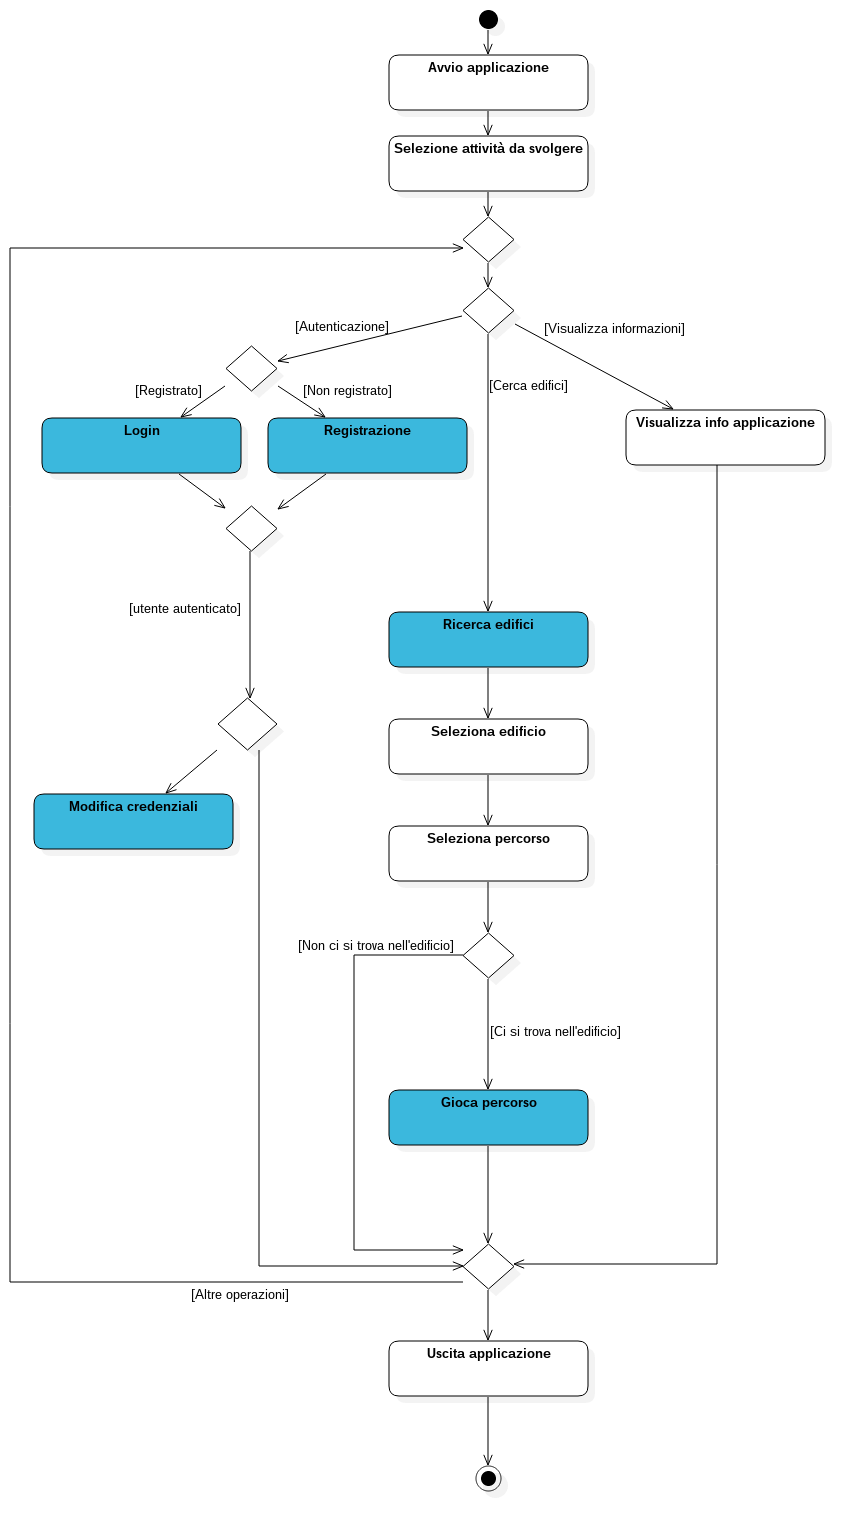
\includegraphics[scale=0.4]{img/attivita/avvio}  
	\caption{Diagramma dell'attività di avvio}
\end{figure}

Questo diagramma contiene tutte le azioni che l'utente può svolgere all'interno dell'applicazione. \\
L'utente può effettuare principalmente tre azioni appena avviata l'applicazione:
\begin{itemize}
	\item \textbf{Autenticarsi}: per autenticarsi l'utente può effettuare la registrazione oppure, se è già registrato, può effettuare il login. Un utente autenticato potrà successivamente modificare le proprie credenziali.
	\item \textbf{Giocare}: l'utente può cercare un edificio nelle vicinanze, successivamente selezionare un edificio, selezionare un percorso e poi giocare. Quest'ultima azione è possibile solo se l'utente si trova nell'edificio che ha selezionato, se così non fosse può uscire dall'applicazione o procedere con altre operazioni.
	\item \textbf{Visualizzare le informazioni relative all'applicazione}: se vuole ricevere informazioni relative all'applicazione l'utente potrà accedere alla schermata apposita accedibile dal menu.
\end{itemize}


\subsection{Registrazione}

\begin{figure}[!h]
	\centering
	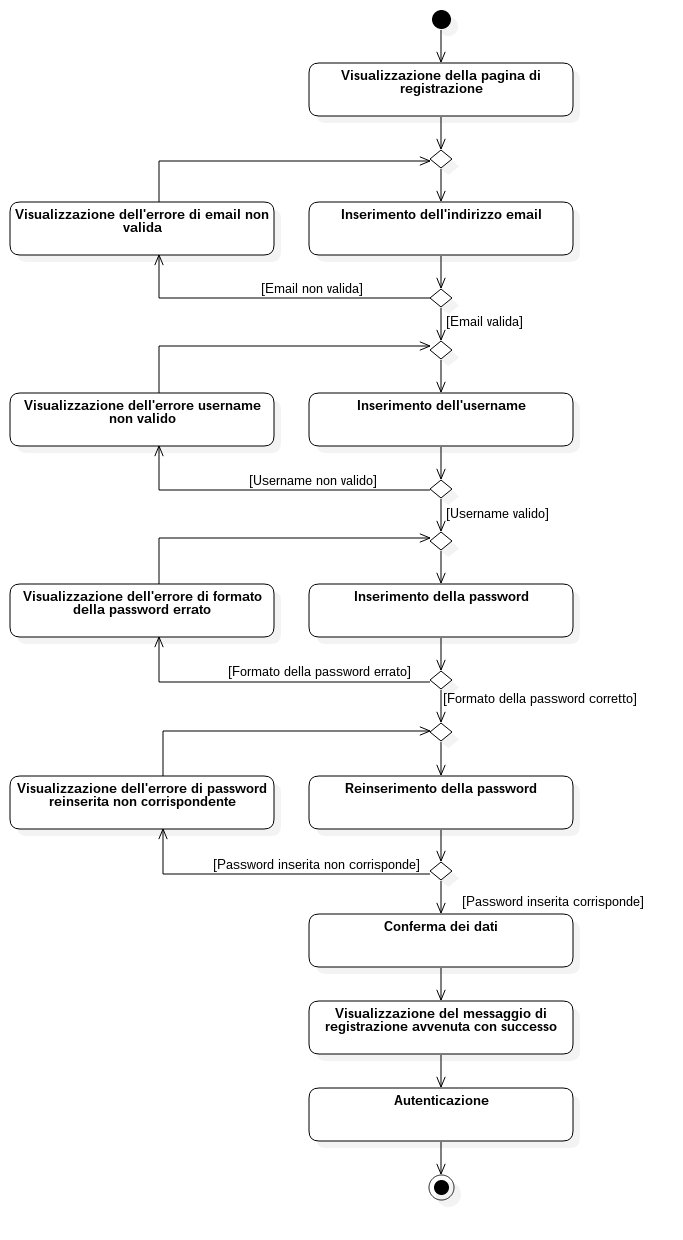
\includegraphics[scale=0.5]{img/attivita/registrazione}  
	\caption{Diagramma dell'attività di registrazione}
\end{figure}

L' utente può registrarsi al sistema inserendo tutti i campi nel form che gli si presenterà davanti una volta cliccato il pulsante ``Registrati'' dal menu dell'applicazione. È previsto l'inserimento obbligatorio di tutti i campi del form.
I campi che l'utente deve riempire sono i seguenti:
\begin{itemize}
	\item Indirizzo email;
	\item Username;
	\item Password;
	\item Reinserimento password;
\end{itemize}
Subito dopo che l'utente riempirà un campo della form verrà subito notificato in caso i dati inseriti non fossero validi. \\
Una volta che tutti i dati saranno inseriti correttamente l'utente potrà confermare i dati e verrà automaticamente autenticato nel sistema.

\newpage

\subsection{Login}

\begin{figure}[!h]
	\centering
	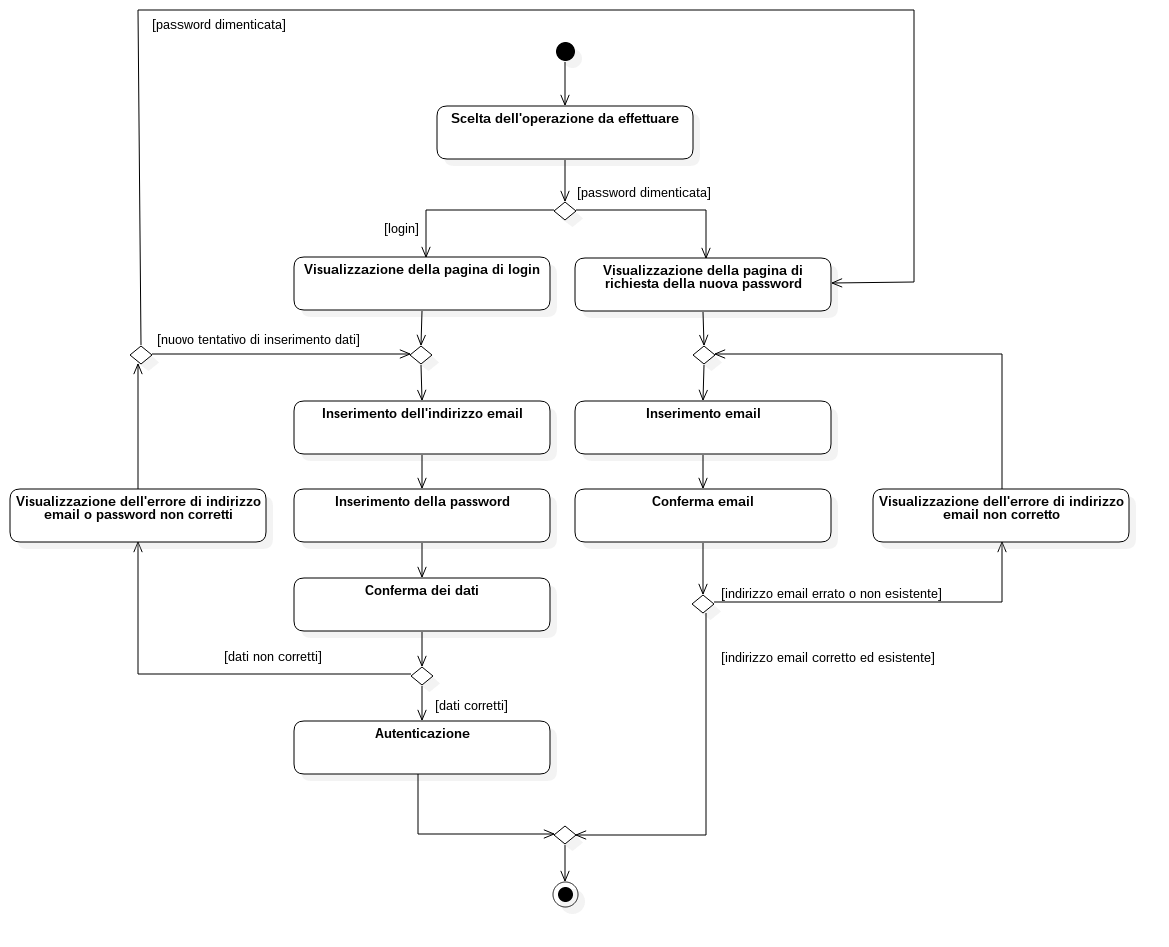
\includegraphics[scale=0.4]{img/attivita/login}  
	\caption{Diagramma dell'attività di login}
\end{figure}

L'utente che si è già registrato e vuole autenticarsi nel sistema deve effettuare il login. \\
Nel caso l'utente ricordi i propri dati per accedere seguirà il ramo sinistro del primo punto di decisione del diagramma. Una volta entrato nella pagina di login inserirà nell'apposito form il proprio indirizzo email e la propria password. Successivamente confermerà i propri dati. Se entrambi i campi sono stati riempiti correttamente l'utente sarà autenticato altrimenti gli viene data l'opportunità di reinserire i dati oppure di effettuare il recupero password. \\
Nel caso l'utente non ricordi le proprie credenziali di accesso può richiedere una nuova password, seguirà quindi il ramo destro del primo punto di decisione del diagramma. Per ottenere una nuova password basterà che inserisca la propria email. Se tale indirizzo è presente nel database del sistema verrà inviata ad esso una email contenente una nuova password. Una volta ricevuta l'email l'utente può tornare nell'applicazione ed effettuare il login seguendo il ramo sinistro del primo punto di decisione del diagramma.

\subsection{Modifica credenzali}

\begin{figure}[!h]
	\centering
	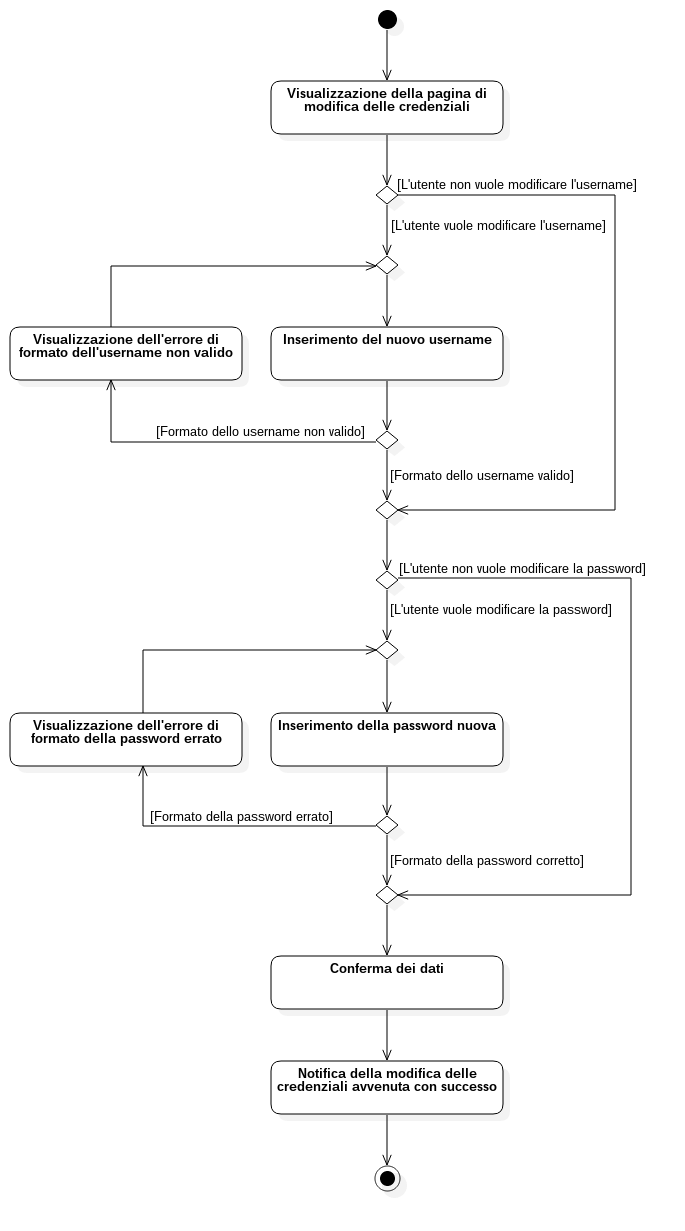
\includegraphics[scale=0.5]{img/attivita/modifica_credenziali}  
	\caption{Diagramma dell'attività di modifica delle credenziali}
\end{figure}

Un utente autenticato può modificare alcune delle sue credenziali. In particolare potrà modificare il proprio username e/o la propria password.
Viene eseguito un controllo di correttezza dei dati inseriti dopo ogni inserimento come avviene durante la registrazione.

\subsection{Percorsi}

\begin{figure}[!h]
	\centering
	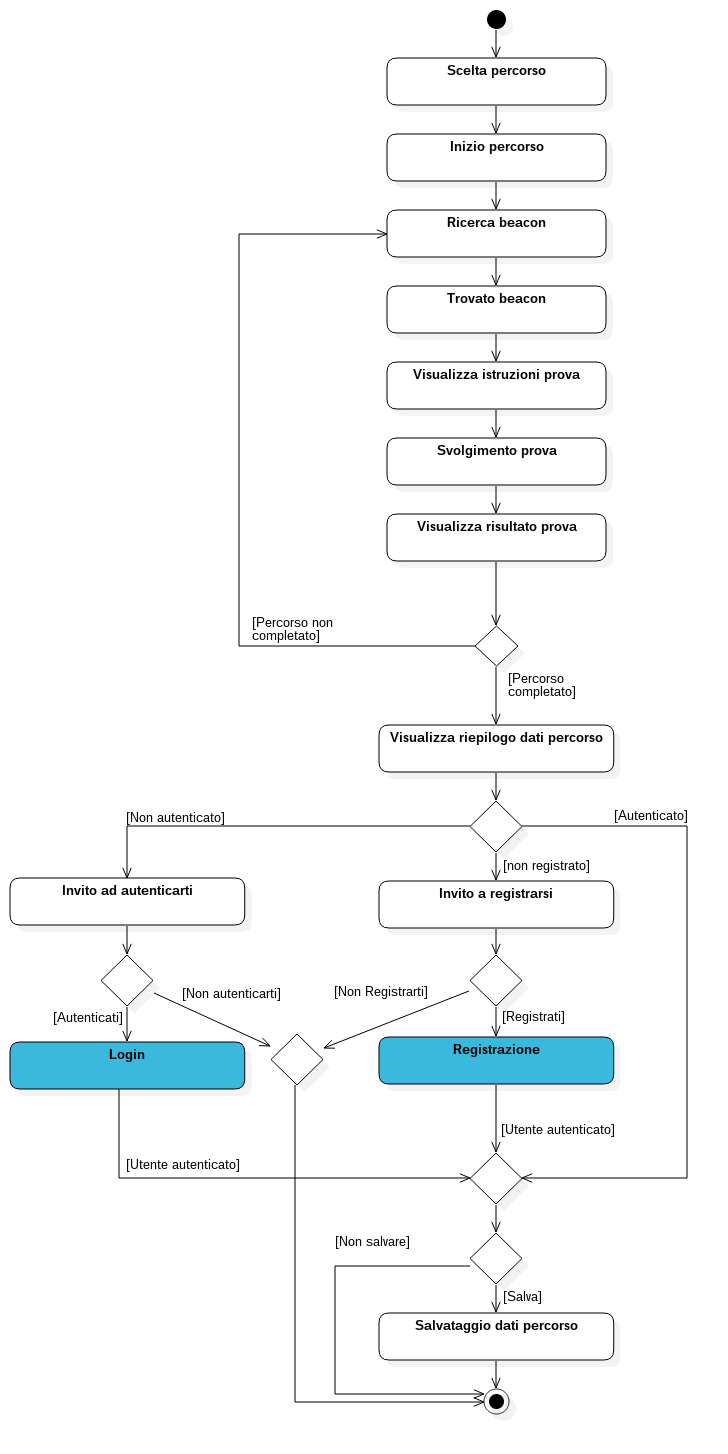
\includegraphics[scale=0.4]{img/attivita/percorsi}  
	\caption{Diagramma dell'attività percorsi}
\end{figure}

Un utente autenticato può decidere di intraprendere un percorso. \\ 
Innanzitutto sceglierà il percorso che desidera fare e successivamente potrà iniziare a svolgerlo. \\ Un percorso si compone di una serie di tappe che prevedono il susseguirsi dei seguenti passi:
\begin{itemize}
	\item Ricerca beacon;
	\item Trovato beacon;
	\item Visualizza istruzioni prova;
	\item Svolgimento prova;
	\item Visualizza risultato prova.
\end{itemize}
L'utente continuerà a svolgere queste azioni finchè il percorso non sarà concluso. Successivamente visualizzerà il riepilogo dei dati del percorso appena concluso e potrà decidere se salvare oppure no i dati che ha appena visualizzato. Quest'ultima operazione sarà possibile solo se l'utente è autenticato, quindi gli viene data la possibilità a questo punto sia di effettuare il login sia di effettuare la registrazione.

\subsection{Ricerca edifici}

\begin{figure}[!h]
	\centering
	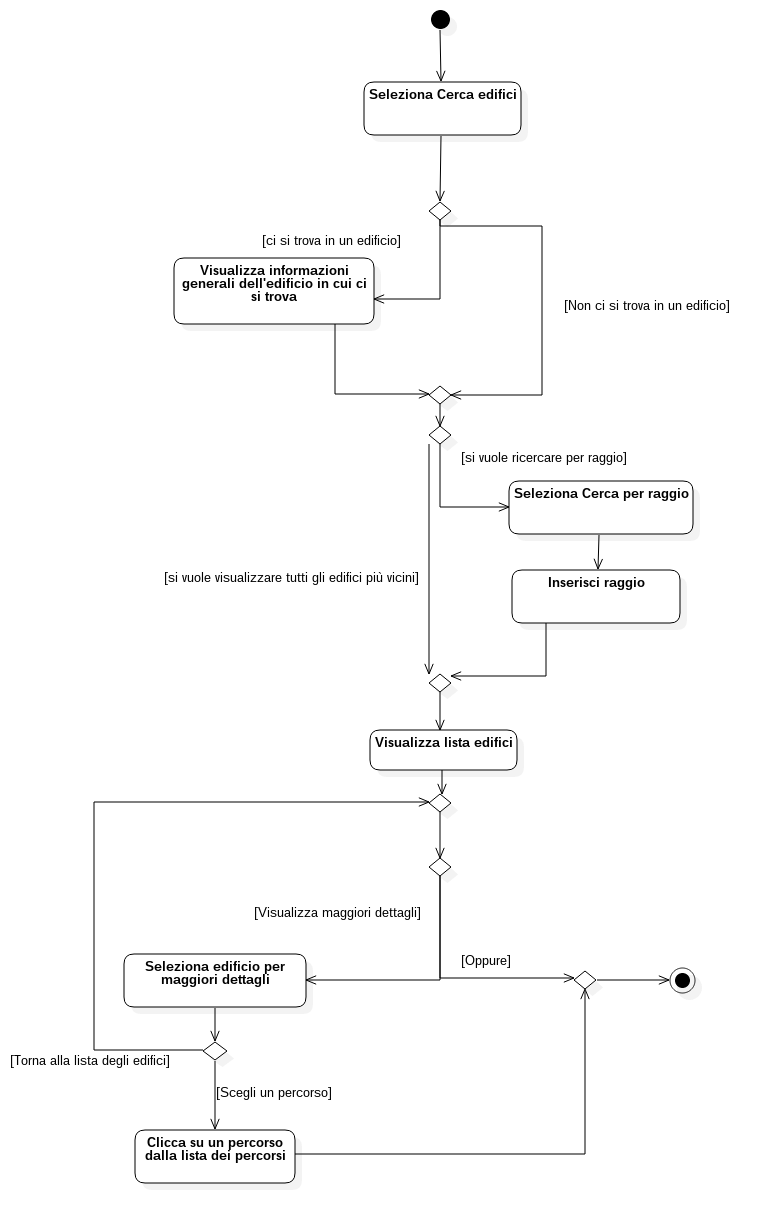
\includegraphics[scale=0.4]{img/attivita/edifici}  
	\caption{Diagramma dell'attività di ricerca edifici}
\end{figure}

L'utente può cercare edifici vicini alla posizione in cui si trova. \\ 
Se si trova in un edificio abilitato visualizzerà direttamente le informazione dell'edificio stesso e successivamente si potrà cercare altri edifici nelle vicinanze. \\ 
Se non si trova in nessun edificio abilitato potrà visualizzare la lista degli edifici più vicini. Se lo desidera si potrà inserire un raggio di ricerca e visualizzare quindi solo gli edifici che gli interessano. \\
Ogni elemento presente nella lista è cliccabile e, una volta cliccato, manderà l'utente in una pagina dove visualizzerà tutti i dettagli dell'edificio e i suoi relativi percorsi.
